\subsection{Organização do projeto}
Antes de iniciar a implementação definiu-se a estrutura do projeto a seguir. \textit{\acrshort{mvc}}foi a estrutura escolhida, uma vez que, é a mais comum e bem estabelecida. Sendo assim, a organização do projeto seguiu a seguinte estrutura:
\begin{figure}[htb]
 \centering
 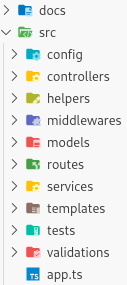
\includegraphics[width=0.2\textwidth]{images/implementacao/api/project_organization.png}
 \caption{Exemplo de página de produto incomum}
 \label{fig:63}
\end{figure}

\begin{itemize}
 \item \textbf{docs} - Documentação gerada;
 \item \textbf{src} - Base de todo o projeto;
 \item \textbf{config} - Ficheiros de configuração do projeto;
 \item \textbf{controllers} - Controladores para cada pedido;
 \item \textbf{helpers} - Ficheiros com funções gerais utilizadas regularmente;
 \item \textbf{middlewares} - Ficheiros com os middlewares da api;
 \item \textbf{models} - Classes criadas para representação de base de dados e outras entidades;
 \item \textbf{routes} - Rotas existentes;
 \item \textbf{services} - Serviços para cada pedido;
 \item \textbf{templates} - Templates de \textit{email} a serem enviados;
 \item \textbf{tests} - Testes de código realizados;
 \item \textbf{validations} - Validações a realizar do modelo de negócio e dos dados;
 \item \textbf{app} - Ficheiro de início do projeto;
\end{itemize}